\section{System Architecture}
\label{sec:arch}

The system has two parts: a Python research pipeline that prepares the data, corrupts inputs, trains and evaluates the variants and produces the reports, and a self-contained browser application that runs the trained baseline and RA-PatchTST side by side. Fig.~\ref{fig:pipeline} shows how data move through the pipeline.

\begin{figure*}[!t]
\centering
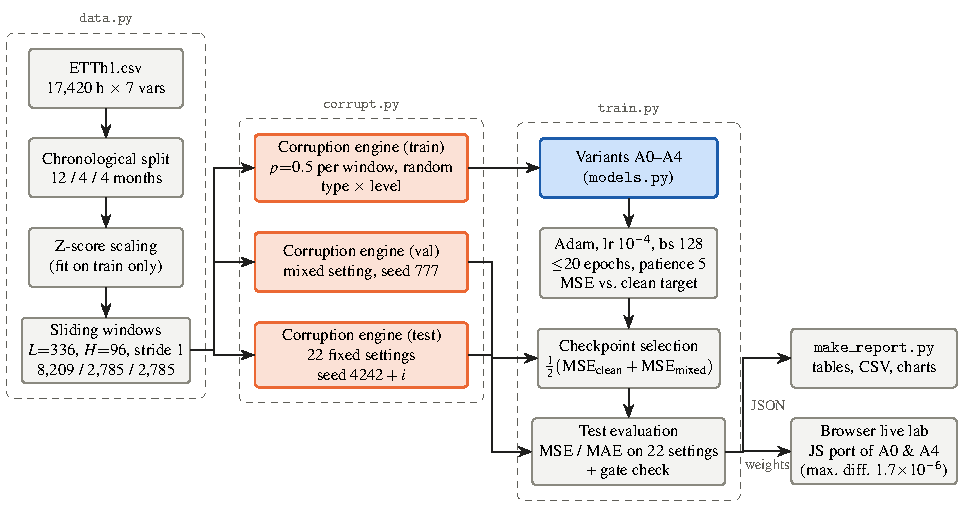
\includegraphics[width=0.92\textwidth]{fig_pipeline.pdf}
\caption{End-to-end pipeline. The same corruption engine produces random corruptions during training, one fixed mixed corruption of the validation set for model selection, and 22 fixed, seeded corruptions of the test set. Results are written as JSON files from which every table and chart is generated; the weights of A0 and A4 are exported to the browser application.}
\label{fig:pipeline}
\end{figure*}

\subsection{Module Design}

The code base consists of five Python modules with narrow interfaces (Table~\ref{tab:modules}). The data module returns tensors only and knows nothing about corruption. The corruption engine is a set of pure functions that take a scaled batch and a seeded random generator and return the corrupted batch together with the mask of altered positions; the same functions serve training, validation and testing, so the corruption seen in evaluation is guaranteed to be the one described in Section~\ref{sec:method-corrupt}. The model module defines a single class whose constructor flags switch the gate and the shift head on or off, and a table that maps each variant name to its flags. The training module owns optimization, selection, evaluation and the gate check, and writes one JSON file per (variant, seed). The report module reads only those JSON files.

\begin{table*}[!t]
\centering
\caption{Software Modules, Responsibilities and Interfaces}
\label{tab:modules}
\footnotesize
\renewcommand{\arraystretch}{1.15}
\begin{tabular}{@{}p{0.14\textwidth}p{0.42\textwidth}p{0.38\textwidth}@{}}
\toprule
Module & Responsibility & Input $\rightarrow$ output \\
\midrule
\texttt{data.py} & Chronological split, train-only scaling, sliding windows, training statistics & CSV file $\rightarrow$ train/val/test tensors, $\bar{\mu}_c,\bar{\sigma}_c$ \\
\texttt{corrupt.py} & Five corruption types, 22 test settings, training-time corruption, patch masks & window batch, seed $\rightarrow$ corrupted batch, mask \\
\texttt{models.py} & PatchTST backbone, reliability gate, shift head; variants A0 to A6 & window batch $\rightarrow$ forecast (and gate weights) \\
\texttt{train.py} & Training loop, checkpoint selection, resumable per-epoch checkpoints, test sweep, gate check & variant, seed $\rightarrow$ result JSON \\
\texttt{make\_report.py} & Aggregation over seeds, tables and charts & result JSON files $\rightarrow$ Markdown, CSV, PNG \\
Live lab (HTML) & JavaScript forward pass of A0 and A4 with embedded weights and test windows & user edits $\rightarrow$ two forecasts, errors, gate weights \\
\bottomrule
\end{tabular}
\end{table*}

\subsection{Tensor Flow Through the Model}

Table~\ref{tab:shapes} traces the shape of the data through one forward pass for a batch of $B$ windows. Channel independence is implemented by folding the channel axis into the batch axis before the encoder and unfolding it before the head; the gate and shift features are computed per channel before folding.

\begin{table}[!t]
\centering
\caption{Tensor Shapes in One Forward Pass}
\label{tab:shapes}
\footnotesize
\colfit{%
\begin{tabular}{@{}ll@{}}
\toprule
Stage & Shape \\
\midrule
Input window $\X$ & $(B,\ 336,\ 7)$ \\
Window statistics $\mu,\sigma$; shift numbers $s^{\mu},s^{\sigma}$ & $(B,\ 7)$ each \\
Patches $\mathbf{p}$ & $(B,\ 7,\ 42,\ 16)$ \\
Gate input $\mathbf{g}$ / gate weights $w$ & $(B,\ 7,\ 42,\ 23)$ / $(B,\ 7,\ 42)$ \\
Embeddings $\mathbf{u}^{(0)}$ (channels folded) & $(7B,\ 42,\ 16)$ \\
Encoder output & $(7B,\ 42,\ 16)$ \\
Head input $[\mathbf{h}_c;s^{\mu}_c;s^{\sigma}_c]$ & $(B,\ 7,\ 674)$ \\
Forecast $\hat{\Y}$ & $(B,\ 96,\ 7)$ \\
\bottomrule
\end{tabular}}
\end{table}

\subsection{Evaluation Subsystem}

Evaluation is deterministic by design. Test setting $i$ ($i=0,\dots,21$) is generated once from the clean test windows with generator seed $4242+i$, and the validation mixed set with seed 777, so all variants and seeds are scored on identical corrupted inputs. For the gated variants the evaluation also reads the gate weights for seven representative settings and splits them by a patch-level mask: a patch counts as corrupted if any of its 16 values was altered, computed by padding and unfolding the position mask exactly as the input is patched.

\subsection{Interactive Live Laboratory}

The live laboratory is a single HTML file that needs no server or network connection. It contains a JavaScript port of the forward pass of A0 and A4 (seed 2021), their trained weights, and a fixed set of 24 ETTh1 test windows. A user picks a window and a channel, applies damage through presets (missing stretches, noise, spikes, level and scale shifts, mixed) or by dragging individual readings, and sees the true future, both forecasts, the damaged input and the trust that the A4 gate gives each patch. A benchmark button runs both models on all $24\times7=168$ sample series under the current damage settings. A dashboard tab shows the experimental results of Section~\ref{sec:results} and states their limitations. When the page was built, the JavaScript forward pass was compared with PyTorch on sample windows and differed by at most $1.7\times10^{-6}$.
